\documentclass[1p]{elsarticle_modified}
%\bibliographystyle{elsarticle-num}

%\usepackage[colorlinks]{hyperref}
%\usepackage{abbrmath_seonhwa} %\Abb, \Ascr, \Acal ,\Abf, \Afrak
\usepackage{amsfonts}
\usepackage{amssymb}
\usepackage{amsmath}
\usepackage{amsthm}
\usepackage{scalefnt}
\usepackage{amsbsy}
\usepackage{kotex}
\usepackage{caption}
\usepackage{subfig}
\usepackage{color}
\usepackage{graphicx}
\usepackage{xcolor} %% white, black, red, green, blue, cyan, magenta, yellow
\usepackage{float}
\usepackage{setspace}
\usepackage{hyperref}

\usepackage{tikz}
\usetikzlibrary{arrows}

\usepackage{multirow}
\usepackage{array} % fixed length table
\usepackage{hhline}

%%%%%%%%%%%%%%%%%%%%%
\makeatletter
\renewcommand*\env@matrix[1][\arraystretch]{%
	\edef\arraystretch{#1}%
	\hskip -\arraycolsep
	\let\@ifnextchar\new@ifnextchar
	\array{*\c@MaxMatrixCols c}}
\makeatother %https://tex.stackexchange.com/questions/14071/how-can-i-increase-the-line-spacing-in-a-matrix
%%%%%%%%%%%%%%%

\usepackage[normalem]{ulem}

\newcommand{\msout}[1]{\ifmmode\text{\sout{\ensuremath{#1}}}\else\sout{#1}\fi}
%SOURCE: \msout is \stkout macro in https://tex.stackexchange.com/questions/20609/strikeout-in-math-mode

\newcommand{\cancel}[1]{
	\ifmmode
	{\color{red}\msout{#1}}
	\else
	{\color{red}\sout{#1}}
	\fi
}

\newcommand{\add}[1]{
	{\color{blue}\uwave{#1}}
}

\newcommand{\replace}[2]{
	\ifmmode
	{\color{red}\msout{#1}}{\color{blue}\uwave{#2}}
	\else
	{\color{red}\sout{#1}}{\color{blue}\uwave{#2}}
	\fi
}

\newcommand{\Sol}{\mathcal{S}} %segment
\newcommand{\D}{D} %diagram
\newcommand{\A}{\mathcal{A}} %arc


%%%%%%%%%%%%%%%%%%%%%%%%%%%%%5 test

\def\sl{\operatorname{\textup{SL}}(2,\Cbb)}
\def\psl{\operatorname{\textup{PSL}}(2,\Cbb)}
\def\quan{\mkern 1mu \triangleright \mkern 1mu}

\theoremstyle{definition}
\newtheorem{thm}{Theorem}[section]
\newtheorem{prop}[thm]{Proposition}
\newtheorem{lem}[thm]{Lemma}
\newtheorem{ques}[thm]{Question}
\newtheorem{cor}[thm]{Corollary}
\newtheorem{defn}[thm]{Definition}
\newtheorem{exam}[thm]{Example}
\newtheorem{rmk}[thm]{Remark}
\newtheorem{alg}[thm]{Algorithm}

\newcommand{\I}{\sqrt{-1}}
\begin{document}

%\begin{frontmatter}
%
%\title{Boundary parabolic representations of knots up to 8 crossings}
%
%%% Group authors per affiliation:
%\author{Yunhi Cho} 
%\address{Department of Mathematics, University of Seoul, Seoul, Korea}
%\ead{yhcho@uos.ac.kr}
%
%
%\author{Seonhwa Kim} %\fnref{s_kim}}
%\address{Center for Geometry and Physics, Institute for Basic Science, Pohang, 37673, Korea}
%\ead{ryeona17@ibs.re.kr}
%
%\author{Hyuk Kim}
%\address{Department of Mathematical Sciences, Seoul National University, Seoul 08826, Korea}
%\ead{hyukkim@snu.ac.kr}
%
%\author{Seokbeom Yoon}
%\address{Department of Mathematical Sciences, Seoul National University, Seoul, 08826,  Korea}
%\ead{sbyoon15@snu.ac.kr}
%
%\begin{abstract}
%We find all boundary parabolic representation of knots up to 8 crossings.
%
%\end{abstract}
%\begin{keyword}
%    \MSC[2010] 57M25 
%\end{keyword}
%
%\end{frontmatter}

%\linenumbers
%\tableofcontents
%
\newcommand\colored[1]{\textcolor{white}{\rule[-0.35ex]{0.8em}{1.4ex}}\kern-0.8em\color{red} #1}%
%\newcommand\colored[1]{\textcolor{white}{ #1}\kern-2.17ex	\textcolor{white}{ #1}\kern-1.81ex	\textcolor{white}{ #1}\kern-2.15ex\color{red}#1	}

{\Large $\underline{12a_{0178}~(K12a_{0178})}$}

\setlength{\tabcolsep}{10pt}
\renewcommand{\arraystretch}{1.6}
\vspace{1cm}\begin{tabular}{m{100pt}>{\centering\arraybackslash}m{274pt}}
\multirow{5}{120pt}{
	\centering
	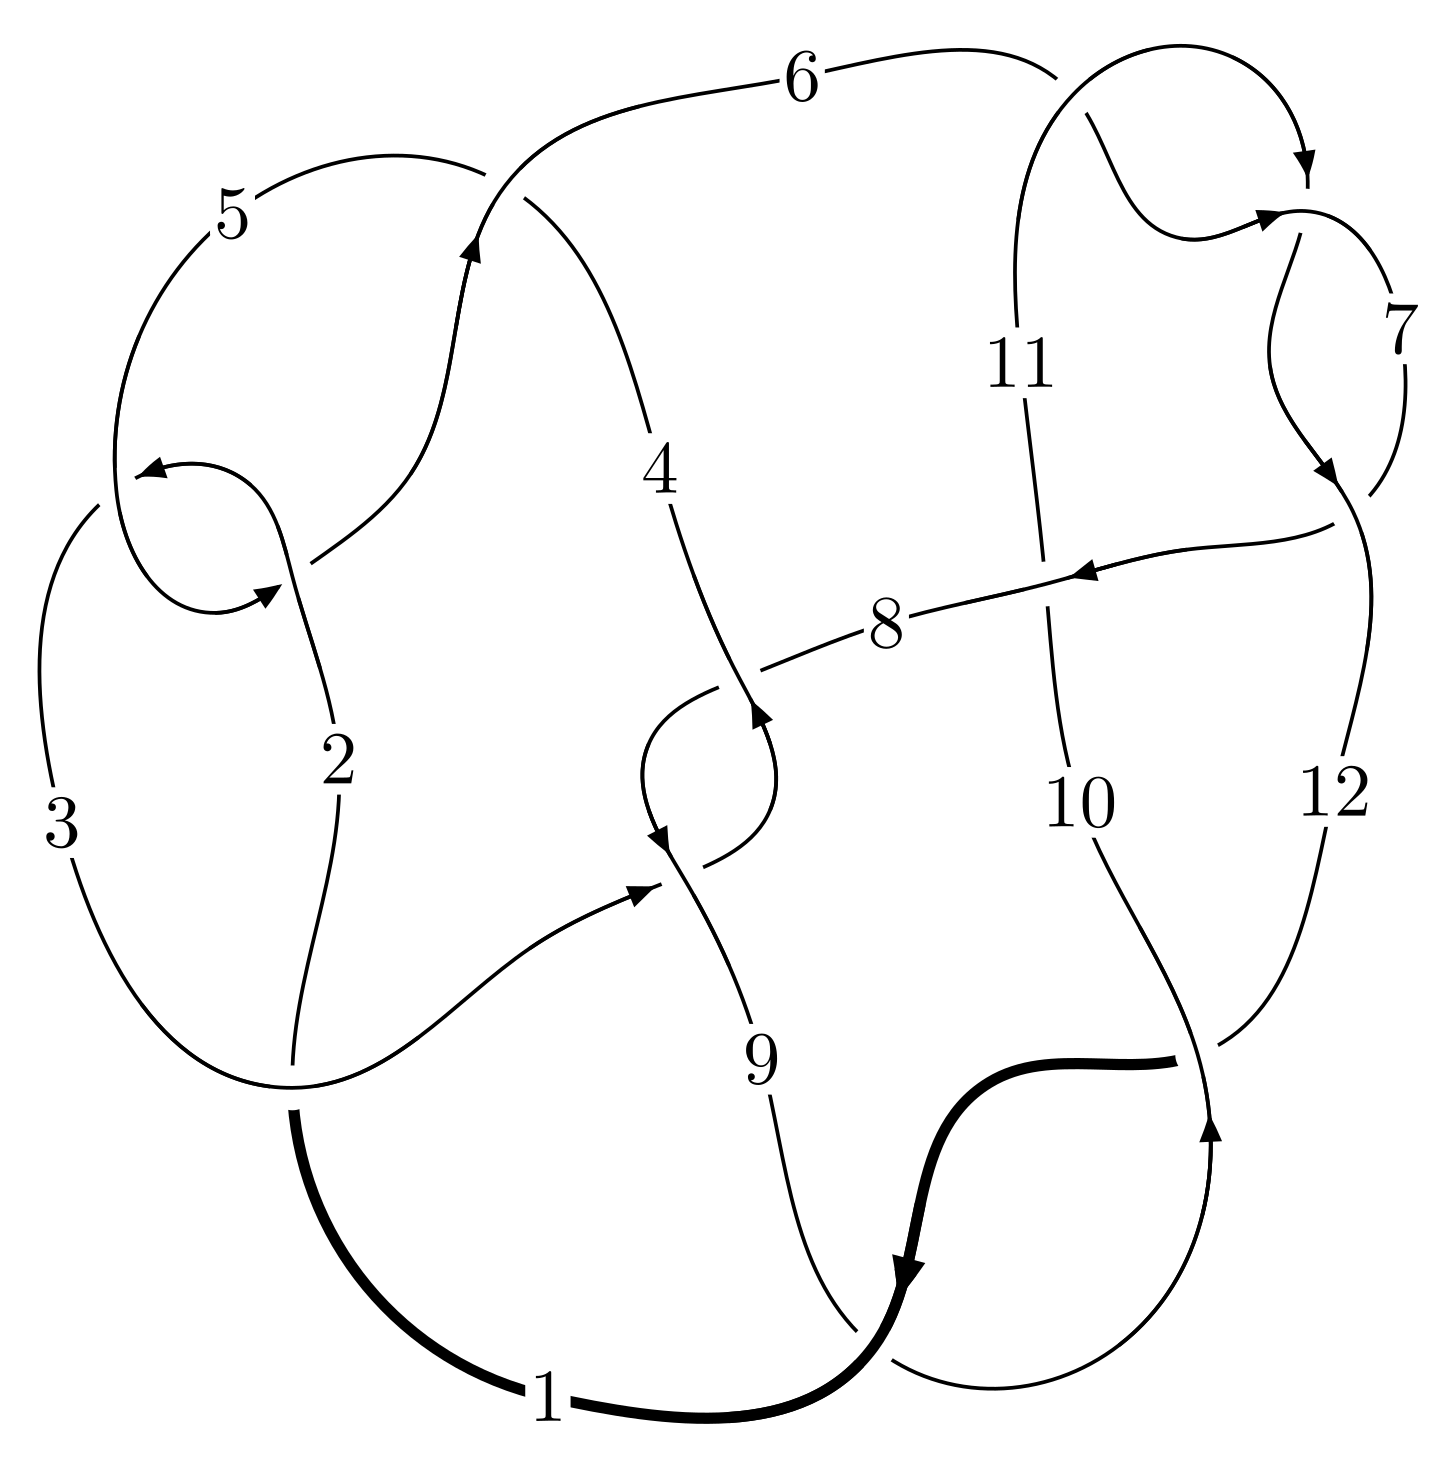
\includegraphics[width=112pt]{../../../GIT/diagram.site/Diagrams/png/979_12a_0178.png}\\
\ \ \ A knot diagram\footnotemark}&
\allowdisplaybreaks
\textbf{Linearized knot diagam} \\
\cline{2-2}
 &
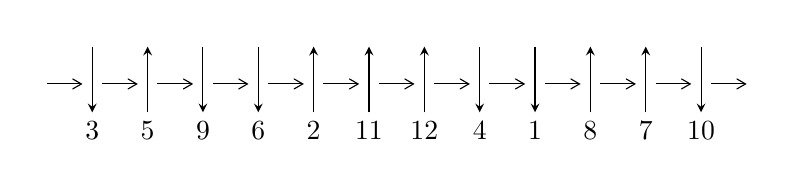
\begin{tikzpicture}[x=20pt, y=17pt]
	% nodes
	\node (C0) at (0, 0) {};
	\node (C1) at (1, 0) {};
	\node (C1U) at (1, +1) {};
	\node (C1D) at (1, -1) {3};

	\node (C2) at (2, 0) {};
	\node (C2U) at (2, +1) {};
	\node (C2D) at (2, -1) {5};

	\node (C3) at (3, 0) {};
	\node (C3U) at (3, +1) {};
	\node (C3D) at (3, -1) {9};

	\node (C4) at (4, 0) {};
	\node (C4U) at (4, +1) {};
	\node (C4D) at (4, -1) {6};

	\node (C5) at (5, 0) {};
	\node (C5U) at (5, +1) {};
	\node (C5D) at (5, -1) {2};

	\node (C6) at (6, 0) {};
	\node (C6U) at (6, +1) {};
	\node (C6D) at (6, -1) {11};

	\node (C7) at (7, 0) {};
	\node (C7U) at (7, +1) {};
	\node (C7D) at (7, -1) {12};

	\node (C8) at (8, 0) {};
	\node (C8U) at (8, +1) {};
	\node (C8D) at (8, -1) {4};

	\node (C9) at (9, 0) {};
	\node (C9U) at (9, +1) {};
	\node (C9D) at (9, -1) {1};

	\node (C10) at (10, 0) {};
	\node (C10U) at (10, +1) {};
	\node (C10D) at (10, -1) {8};

	\node (C11) at (11, 0) {};
	\node (C11U) at (11, +1) {};
	\node (C11D) at (11, -1) {7};

	\node (C12) at (12, 0) {};
	\node (C12U) at (12, +1) {};
	\node (C12D) at (12, -1) {10};
	\node (C13) at (13, 0) {};

	% arrows
	\draw[->,>={angle 60}]
	(C0) edge (C1) (C1) edge (C2) (C2) edge (C3) (C3) edge (C4) (C4) edge (C5) (C5) edge (C6) (C6) edge (C7) (C7) edge (C8) (C8) edge (C9) (C9) edge (C10) (C10) edge (C11) (C11) edge (C12) (C12) edge (C13) ;	\draw[->,>=stealth]
	(C1U) edge (C1D) (C2D) edge (C2U) (C3U) edge (C3D) (C4U) edge (C4D) (C5D) edge (C5U) (C6D) edge (C6U) (C7D) edge (C7U) (C8U) edge (C8D) (C9U) edge (C9D) (C10D) edge (C10U) (C11D) edge (C11U) (C12U) edge (C12D) ;
	\end{tikzpicture} \\
\hhline{~~} \\& 
\textbf{Solving Sequence} \\ \cline{2-2} 
 &
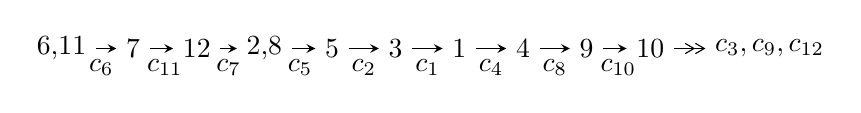
\begin{tikzpicture}[x=23pt, y=7pt]
	% node
	\node (A0) at (-1/8, 0) {6,11};
	\node (A1) at (1, 0) {7};
	\node (A2) at (2, 0) {12};
	\node (A3) at (49/16, 0) {2,8};
	\node (A4) at (33/8, 0) {5};
	\node (A5) at (41/8, 0) {3};
	\node (A6) at (49/8, 0) {1};
	\node (A7) at (57/8, 0) {4};
	\node (A8) at (65/8, 0) {9};
	\node (A9) at (73/8, 0) {10};
	\node (C1) at (1/2, -1) {$c_{6}$};
	\node (C2) at (3/2, -1) {$c_{11}$};
	\node (C3) at (5/2, -1) {$c_{7}$};
	\node (C4) at (29/8, -1) {$c_{5}$};
	\node (C5) at (37/8, -1) {$c_{2}$};
	\node (C6) at (45/8, -1) {$c_{1}$};
	\node (C7) at (53/8, -1) {$c_{4}$};
	\node (C8) at (61/8, -1) {$c_{8}$};
	\node (C9) at (69/8, -1) {$c_{10}$};
	\node (A10) at (11, 0) {$c_{3},c_{9},c_{12}$};

	% edge
	\draw[->,>=stealth]	
	(A0) edge (A1) (A1) edge (A2) (A2) edge (A3) (A3) edge (A4) (A4) edge (A5) (A5) edge (A6) (A6) edge (A7) (A7) edge (A8) (A8) edge (A9) ;
	\draw[->>,>={angle 60}]	
	(A9) edge (A10);
\end{tikzpicture} \\ 

\end{tabular} \\

\footnotetext{
The image of knot diagram is generated by the software ``\textbf{Draw programme}" developed by Andrew Bartholomew(\url{http://www.layer8.co.uk/maths/draw/index.htm\#Running-draw}), where we modified some parts for our purpose(\url{https://github.com/CATsTAILs/LinksPainter}).
}\phantom \\ \newline 
\centering \textbf{Ideals for irreducible components\footnotemark of $X_{\text{par}}$} 
 
\begin{align*}
I^u_{1}&=\langle 
u^{76}- u^{75}+\cdots+2 b-5 u,\;2 u^{78}-4 u^{77}+\cdots+2 a-1,\;u^{79}-3 u^{78}+\cdots+u-1\rangle \\
I^u_{2}&=\langle 
u^3 a+u^3- a u+b- a- u-1,\;- u^3 a- u^4+a^2+2 a u+2 u^2+2 a,\;u^5- u^4-2 u^3+u^2+u+1\rangle \\
\\
\end{align*}
\raggedright * 2 irreducible components of $\dim_{\mathbb{C}}=0$, with total 89 representations.\\
\footnotetext{All coefficients of polynomials are rational numbers. But the coefficients are sometimes approximated in decimal forms when there is not enough margin.}
\newpage
\renewcommand{\arraystretch}{1}
\centering \section*{I. $I^u_{1}= \langle u^{76}- u^{75}+\cdots+2 b-5 u,\;2 u^{78}-4 u^{77}+\cdots+2 a-1,\;u^{79}-3 u^{78}+\cdots+u-1 \rangle$}
\flushleft \textbf{(i) Arc colorings}\\
\begin{tabular}{m{7pt} m{180pt} m{7pt} m{180pt} }
\flushright $a_{6}=$&$\begin{pmatrix}1\\0\end{pmatrix}$ \\
\flushright $a_{11}=$&$\begin{pmatrix}0\\u\end{pmatrix}$ \\
\flushright $a_{7}=$&$\begin{pmatrix}1\\- u^2\end{pmatrix}$ \\
\flushright $a_{12}=$&$\begin{pmatrix}u\\- u^3+u\end{pmatrix}$ \\
\flushright $a_{2}=$&$\begin{pmatrix}- u^{78}+2 u^{77}+\cdots-\frac{3}{2} u+\frac{1}{2}\\-\frac{1}{2} u^{76}+\frac{1}{2} u^{75}+\cdots-\frac{11}{2} u^2+\frac{5}{2} u\end{pmatrix}$ \\
\flushright $a_{8}=$&$\begin{pmatrix}- u^2+1\\u^4-2 u^2\end{pmatrix}$ \\
\flushright $a_{5}=$&$\begin{pmatrix}-2 u^{78}+4 u^{77}+\cdots+5 u-\frac{1}{2}\\3 u^{78}-5 u^{77}+\cdots+\frac{3}{2} u+1\end{pmatrix}$ \\
\flushright $a_{3}=$&$\begin{pmatrix}-5 u^{78}+8 u^{77}+\cdots+\frac{17}{2} u-\frac{5}{2}\\5 u^{78}-8 u^{77}+\cdots+\frac{3}{2} u+2\end{pmatrix}$ \\
\flushright $a_{1}=$&$\begin{pmatrix}u^9-4 u^7+5 u^5-2 u^3+u\\- u^{11}+5 u^9-8 u^7+3 u^5+u^3+u\end{pmatrix}$ \\
\flushright $a_{4}=$&$\begin{pmatrix}u^{78}- u^{77}+\cdots+\frac{13}{2} u+\frac{1}{2}\\3 u^{78}-5 u^{77}+\cdots+\frac{3}{2} u+1\end{pmatrix}$ \\
\flushright $a_{9}=$&$\begin{pmatrix}u^{13}-6 u^{11}+13 u^9-12 u^7+6 u^5-4 u^3+u\\- u^{15}+7 u^{13}-18 u^{11}+19 u^9-6 u^7+2 u^5-4 u^3- u\end{pmatrix}$ \\
\flushright $a_{10}=$&$\begin{pmatrix}- u^5+2 u^3- u\\u^7-3 u^5+2 u^3+u\end{pmatrix}$\\&\end{tabular}
\flushleft \textbf{(ii) Obstruction class $= -1$}\\~\\
\flushleft \textbf{(iii) Cusp Shapes $= \frac{11}{2} u^{78}-\frac{19}{2} u^{77}+\cdots-22 u+\frac{3}{2}$}\\~\\
\newpage\renewcommand{\arraystretch}{1}
\flushleft \textbf{(iv) u-Polynomials at the component}\newline \\
\begin{tabular}{m{50pt}|m{274pt}}
Crossings & \hspace{64pt}u-Polynomials at each crossing \\
\hline $$\begin{aligned}c_{1},c_{4}\end{aligned}$$&$\begin{aligned}
&u^{79}+24 u^{78}+\cdots-14 u-1
\end{aligned}$\\
\hline $$\begin{aligned}c_{2},c_{5}\end{aligned}$$&$\begin{aligned}
&u^{79}+6 u^{78}+\cdots+2 u+1
\end{aligned}$\\
\hline $$\begin{aligned}c_{3},c_{8}\end{aligned}$$&$\begin{aligned}
&u^{79}+u^{78}+\cdots-2048 u-1024
\end{aligned}$\\
\hline $$\begin{aligned}c_{6},c_{7},c_{11}\end{aligned}$$&$\begin{aligned}
&u^{79}-3 u^{78}+\cdots+u-1
\end{aligned}$\\
\hline $$\begin{aligned}c_{9},c_{12}\end{aligned}$$&$\begin{aligned}
&u^{79}-11 u^{78}+\cdots-117 u-73
\end{aligned}$\\
\hline $$\begin{aligned}c_{10}\end{aligned}$$&$\begin{aligned}
&u^{79}+9 u^{78}+\cdots-2487 u+851
\end{aligned}$\\
\hline
\end{tabular}\\~\\
\newpage\renewcommand{\arraystretch}{1}
\flushleft \textbf{(v) Riley Polynomials at the component}\newline \\
\begin{tabular}{m{50pt}|m{274pt}}
Crossings & \hspace{64pt}Riley Polynomials at each crossing \\
\hline $$\begin{aligned}c_{1},c_{4}\end{aligned}$$&$\begin{aligned}
&y^{79}+68 y^{78}+\cdots+270 y-1
\end{aligned}$\\
\hline $$\begin{aligned}c_{2},c_{5}\end{aligned}$$&$\begin{aligned}
&y^{79}+24 y^{78}+\cdots-14 y-1
\end{aligned}$\\
\hline $$\begin{aligned}c_{3},c_{8}\end{aligned}$$&$\begin{aligned}
&y^{79}+55 y^{78}+\cdots-9437184 y-1048576
\end{aligned}$\\
\hline $$\begin{aligned}c_{6},c_{7},c_{11}\end{aligned}$$&$\begin{aligned}
&y^{79}-75 y^{78}+\cdots-23 y-1
\end{aligned}$\\
\hline $$\begin{aligned}c_{9},c_{12}\end{aligned}$$&$\begin{aligned}
&y^{79}+73 y^{78}+\cdots-70115 y-5329
\end{aligned}$\\
\hline $$\begin{aligned}c_{10}\end{aligned}$$&$\begin{aligned}
&y^{79}-31 y^{78}+\cdots-2637999 y-724201
\end{aligned}$\\
\hline
\end{tabular}\\~\\
\newpage\flushleft \textbf{(vi) Complex Volumes and Cusp Shapes}
$$\begin{array}{c|c|c}  
\text{Solutions to }I^u_{1}& \I (\text{vol} + \sqrt{-1}CS) & \text{Cusp shape}\\
 \hline 
\begin{aligned}
u &= \phantom{-}0.960687 + 0.153679 I \\
a &= \phantom{-}0.507114 + 0.208480 I \\
b &= -0.750208 + 0.893053 I\end{aligned}
 & \phantom{-}4.67325 - 2.88323 I & \phantom{-0.000000 } 0 \\ \hline\begin{aligned}
u &= \phantom{-}0.960687 - 0.153679 I \\
a &= \phantom{-}0.507114 - 0.208480 I \\
b &= -0.750208 - 0.893053 I\end{aligned}
 & \phantom{-}4.67325 + 2.88323 I & \phantom{-0.000000 } 0 \\ \hline\begin{aligned}
u &= \phantom{-}0.827370 + 0.170912 I \\
a &= \phantom{-}0.960753 - 0.367241 I \\
b &= -0.764781 - 0.869204 I\end{aligned}
 & \phantom{-}4.74752 + 2.85194 I & \phantom{-}5.96777 - 3.55563 I \\ \hline\begin{aligned}
u &= \phantom{-}0.827370 - 0.170912 I \\
a &= \phantom{-}0.960753 + 0.367241 I \\
b &= -0.764781 + 0.869204 I\end{aligned}
 & \phantom{-}4.74752 - 2.85194 I & \phantom{-}5.96777 + 3.55563 I \\ \hline\begin{aligned}
u &= -0.431098 + 0.703014 I \\
a &= -0.011403 + 1.045270 I \\
b &= -0.906120 - 0.737961 I\end{aligned}
 & \phantom{-}9.87956 - 5.56873 I & \phantom{-}5.48276 + 3.81380 I \\ \hline\begin{aligned}
u &= -0.431098 - 0.703014 I \\
a &= -0.011403 - 1.045270 I \\
b &= -0.906120 + 0.737961 I\end{aligned}
 & \phantom{-}9.87956 + 5.56873 I & \phantom{-}5.48276 - 3.81380 I \\ \hline\begin{aligned}
u &= -0.417770 + 0.709165 I \\
a &= \phantom{-}2.06985 + 1.21835 I \\
b &= -0.786589 + 1.032560 I\end{aligned}
 & \phantom{-}8.9584 - 11.8257 I & \phantom{-}3.97751 + 8.54937 I \\ \hline\begin{aligned}
u &= -0.417770 - 0.709165 I \\
a &= \phantom{-}2.06985 - 1.21835 I \\
b &= -0.786589 - 1.032560 I\end{aligned}
 & \phantom{-}8.9584 + 11.8257 I & \phantom{-}3.97751 - 8.54937 I \\ \hline\begin{aligned}
u &= -0.541357 + 0.617925 I \\
a &= \phantom{-}1.260830 + 0.092818 I \\
b &= -0.902271 + 0.758090 I\end{aligned}
 & \phantom{-}10.28590 + 1.15255 I & \phantom{-}6.41028 + 2.08924 I \\ \hline\begin{aligned}
u &= -0.541357 - 0.617925 I \\
a &= \phantom{-}1.260830 - 0.092818 I \\
b &= -0.902271 - 0.758090 I\end{aligned}
 & \phantom{-}10.28590 - 1.15255 I & \phantom{-}6.41028 - 2.08924 I\\
 \hline 
 \end{array}$$\newpage$$\begin{array}{c|c|c}  
\text{Solutions to }I^u_{1}& \I (\text{vol} + \sqrt{-1}CS) & \text{Cusp shape}\\
 \hline 
\begin{aligned}
u &= -0.554854 + 0.602818 I \\
a &= \phantom{-}0.818220 + 0.193142 I \\
b &= -0.794943 - 1.020680 I\end{aligned}
 & \phantom{-}9.46345 + 7.42771 I & \phantom{-}5.21274 - 2.74453 I \\ \hline\begin{aligned}
u &= -0.554854 - 0.602818 I \\
a &= \phantom{-}0.818220 - 0.193142 I \\
b &= -0.794943 + 1.020680 I\end{aligned}
 & \phantom{-}9.46345 - 7.42771 I & \phantom{-}5.21274 + 2.74453 I \\ \hline\begin{aligned}
u &= -0.460232 + 0.639959 I \\
a &= -0.538335 - 0.631341 I \\
b &= \phantom{-}0.819242 - 0.023424 I\end{aligned}
 & \phantom{-}5.68856 - 2.11060 I & \phantom{-}6.83378 + 3.31832 I \\ \hline\begin{aligned}
u &= -0.460232 - 0.639959 I \\
a &= -0.538335 + 0.631341 I \\
b &= \phantom{-}0.819242 + 0.023424 I\end{aligned}
 & \phantom{-}5.68856 + 2.11060 I & \phantom{-}6.83378 - 3.31832 I \\ \hline\begin{aligned}
u &= \phantom{-}0.446094 + 0.644815 I \\
a &= -2.25296 + 0.31798 I \\
b &= \phantom{-}0.776837 + 0.897829 I\end{aligned}
 & \phantom{-}4.79648 + 5.02800 I & \phantom{-}3.77738 - 5.92269 I \\ \hline\begin{aligned}
u &= \phantom{-}0.446094 - 0.644815 I \\
a &= -2.25296 - 0.31798 I \\
b &= \phantom{-}0.776837 - 0.897829 I\end{aligned}
 & \phantom{-}4.79648 - 5.02800 I & \phantom{-}3.77738 + 5.92269 I \\ \hline\begin{aligned}
u &= \phantom{-}1.211160 + 0.128664 I \\
a &= \phantom{-}1.28344 - 1.04569 I \\
b &= \phantom{-}0.018725 - 0.877436 I\end{aligned}
 & \phantom{-}0.410093 + 0.569090 I & \phantom{-0.000000 } 0 \\ \hline\begin{aligned}
u &= \phantom{-}1.211160 - 0.128664 I \\
a &= \phantom{-}1.28344 + 1.04569 I \\
b &= \phantom{-}0.018725 + 0.877436 I\end{aligned}
 & \phantom{-}0.410093 - 0.569090 I & \phantom{-0.000000 } 0 \\ \hline\begin{aligned}
u &= \phantom{-}0.465338 + 0.625622 I \\
a &= -0.819821 + 1.071380 I \\
b &= \phantom{-}0.783132 - 0.871429 I\end{aligned}
 & \phantom{-}4.87790 - 0.84564 I & \phantom{-}4.12547 - 0.52207 I \\ \hline\begin{aligned}
u &= \phantom{-}0.465338 - 0.625622 I \\
a &= -0.819821 - 1.071380 I \\
b &= \phantom{-}0.783132 + 0.871429 I\end{aligned}
 & \phantom{-}4.87790 + 0.84564 I & \phantom{-}4.12547 + 0.52207 I\\
 \hline 
 \end{array}$$\newpage$$\begin{array}{c|c|c}  
\text{Solutions to }I^u_{1}& \I (\text{vol} + \sqrt{-1}CS) & \text{Cusp shape}\\
 \hline 
\begin{aligned}
u &= -0.416187 + 0.649698 I \\
a &= -1.47061 - 1.27515 I \\
b &= \phantom{-}0.281669 - 1.127160 I\end{aligned}
 & \phantom{-}1.81369 - 5.81158 I & \phantom{-}1.46444 + 7.37025 I \\ \hline\begin{aligned}
u &= -0.416187 - 0.649698 I \\
a &= -1.47061 + 1.27515 I \\
b &= \phantom{-}0.281669 + 1.127160 I\end{aligned}
 & \phantom{-}1.81369 + 5.81158 I & \phantom{-}1.46444 - 7.37025 I \\ \hline\begin{aligned}
u &= -0.467486 + 0.588976 I \\
a &= \phantom{-}0.271507 + 0.612178 I \\
b &= \phantom{-}0.318145 + 1.112630 I\end{aligned}
 & \phantom{-}2.05435 + 1.75127 I & \phantom{-}2.62331 - 0.74126 I \\ \hline\begin{aligned}
u &= -0.467486 - 0.588976 I \\
a &= \phantom{-}0.271507 - 0.612178 I \\
b &= \phantom{-}0.318145 - 1.112630 I\end{aligned}
 & \phantom{-}2.05435 - 1.75127 I & \phantom{-}2.62331 + 0.74126 I \\ \hline\begin{aligned}
u &= \phantom{-}1.26366\phantom{ +0.000000I} \\
a &= \phantom{-}0.931332\phantom{ +0.000000I} \\
b &= -0.238856\phantom{ +0.000000I}\end{aligned}
 & \phantom{-}2.75626\phantom{ +0.000000I} & \phantom{-0.000000 } 0 \\ \hline\begin{aligned}
u &= \phantom{-}0.174701 + 0.686237 I \\
a &= -0.699194 + 0.373449 I \\
b &= -0.764897 + 0.812003 I\end{aligned}
 & \phantom{-}2.54707 + 0.60070 I & \phantom{-}2.16281 - 1.57893 I \\ \hline\begin{aligned}
u &= \phantom{-}0.174701 - 0.686237 I \\
a &= -0.699194 - 0.373449 I \\
b &= -0.764897 - 0.812003 I\end{aligned}
 & \phantom{-}2.54707 - 0.60070 I & \phantom{-}2.16281 + 1.57893 I \\ \hline\begin{aligned}
u &= \phantom{-}0.140244 + 0.692618 I \\
a &= \phantom{-}0.66990 - 1.89405 I \\
b &= -0.742698 - 0.939246 I\end{aligned}
 & \phantom{-}2.15562 + 6.31590 I & \phantom{-}0.72997 - 6.99064 I \\ \hline\begin{aligned}
u &= \phantom{-}0.140244 - 0.692618 I \\
a &= \phantom{-}0.66990 + 1.89405 I \\
b &= -0.742698 + 0.939246 I\end{aligned}
 & \phantom{-}2.15562 - 6.31590 I & \phantom{-}0.72997 + 6.99064 I \\ \hline\begin{aligned}
u &= \phantom{-}0.331444 + 0.619754 I \\
a &= \phantom{-}1.70156 - 0.90801 I \\
b &= -0.146875 - 0.718790 I\end{aligned}
 & -0.39859 + 2.41679 I & -2.51815 - 2.50379 I\\
 \hline 
 \end{array}$$\newpage$$\begin{array}{c|c|c}  
\text{Solutions to }I^u_{1}& \I (\text{vol} + \sqrt{-1}CS) & \text{Cusp shape}\\
 \hline 
\begin{aligned}
u &= \phantom{-}0.331444 - 0.619754 I \\
a &= \phantom{-}1.70156 + 0.90801 I \\
b &= -0.146875 + 0.718790 I\end{aligned}
 & -0.39859 - 2.41679 I & -2.51815 + 2.50379 I \\ \hline\begin{aligned}
u &= -1.284980 + 0.179165 I \\
a &= -0.74042 - 1.23710 I \\
b &= \phantom{-}0.156711 - 1.014790 I\end{aligned}
 & \phantom{-}1.15848 - 4.83085 I & \phantom{-0.000000 } 0 \\ \hline\begin{aligned}
u &= -1.284980 - 0.179165 I \\
a &= -0.74042 + 1.23710 I \\
b &= \phantom{-}0.156711 + 1.014790 I\end{aligned}
 & \phantom{-}1.15848 + 4.83085 I & \phantom{-0.000000 } 0 \\ \hline\begin{aligned}
u &= -1.300270 + 0.074806 I \\
a &= -0.754795 + 0.685987 I \\
b &= \phantom{-}0.494882 + 1.001490 I\end{aligned}
 & \phantom{-}3.08759 + 1.25662 I & \phantom{-0.000000 } 0 \\ \hline\begin{aligned}
u &= -1.300270 - 0.074806 I \\
a &= -0.754795 - 0.685987 I \\
b &= \phantom{-}0.494882 - 1.001490 I\end{aligned}
 & \phantom{-}3.08759 - 1.25662 I & \phantom{-0.000000 } 0 \\ \hline\begin{aligned}
u &= -1.311810 + 0.262394 I \\
a &= \phantom{-}1.97615 + 0.97895 I \\
b &= -0.742423 + 0.968481 I\end{aligned}
 & \phantom{-}6.68975 - 9.77430 I & \phantom{-0.000000 } 0 \\ \hline\begin{aligned}
u &= -1.311810 - 0.262394 I \\
a &= \phantom{-}1.97615 - 0.97895 I \\
b &= -0.742423 - 0.968481 I\end{aligned}
 & \phantom{-}6.68975 + 9.77430 I & \phantom{-0.000000 } 0 \\ \hline\begin{aligned}
u &= \phantom{-}1.330220 + 0.148111 I \\
a &= -2.77349 + 0.42700 I \\
b &= \phantom{-}0.643454 + 0.948330 I\end{aligned}
 & \phantom{-}4.02017 + 5.12137 I & \phantom{-0.000000 } 0 \\ \hline\begin{aligned}
u &= \phantom{-}1.330220 - 0.148111 I \\
a &= -2.77349 - 0.42700 I \\
b &= \phantom{-}0.643454 - 0.948330 I\end{aligned}
 & \phantom{-}4.02017 - 5.12137 I & \phantom{-0.000000 } 0 \\ \hline\begin{aligned}
u &= \phantom{-}1.345390 + 0.105400 I \\
a &= -0.77119 + 1.72286 I \\
b &= \phantom{-}0.672238 - 0.709217 I\end{aligned}
 & \phantom{-}4.74837 + 0.02263 I & \phantom{-0.000000 } 0\\
 \hline 
 \end{array}$$\newpage$$\begin{array}{c|c|c}  
\text{Solutions to }I^u_{1}& \I (\text{vol} + \sqrt{-1}CS) & \text{Cusp shape}\\
 \hline 
\begin{aligned}
u &= \phantom{-}1.345390 - 0.105400 I \\
a &= -0.77119 - 1.72286 I \\
b &= \phantom{-}0.672238 + 0.709217 I\end{aligned}
 & \phantom{-}4.74837 - 0.02263 I & \phantom{-0.000000 } 0 \\ \hline\begin{aligned}
u &= -1.354000 + 0.125122 I \\
a &= -0.577117 + 0.093747 I \\
b &= \phantom{-}0.589160 - 0.295718 I\end{aligned}
 & \phantom{-}5.02105 - 2.84369 I & \phantom{-0.000000 } 0 \\ \hline\begin{aligned}
u &= -1.354000 - 0.125122 I \\
a &= -0.577117 - 0.093747 I \\
b &= \phantom{-}0.589160 + 0.295718 I\end{aligned}
 & \phantom{-}5.02105 + 2.84369 I & \phantom{-0.000000 } 0 \\ \hline\begin{aligned}
u &= -1.336080 + 0.257261 I \\
a &= \phantom{-}0.095226 + 0.877787 I \\
b &= -0.779371 - 0.771197 I\end{aligned}
 & \phantom{-}7.28961 - 4.01466 I & \phantom{-0.000000 } 0 \\ \hline\begin{aligned}
u &= -1.336080 - 0.257261 I \\
a &= \phantom{-}0.095226 - 0.877787 I \\
b &= -0.779371 + 0.771197 I\end{aligned}
 & \phantom{-}7.28961 + 4.01466 I & \phantom{-0.000000 } 0 \\ \hline\begin{aligned}
u &= \phantom{-}0.055935 + 0.584888 I \\
a &= \phantom{-}0.34048 + 2.64860 I \\
b &= \phantom{-}0.118978 + 0.935231 I\end{aligned}
 & -2.96390 + 2.06663 I & -7.76438 - 4.75095 I \\ \hline\begin{aligned}
u &= \phantom{-}0.055935 - 0.584888 I \\
a &= \phantom{-}0.34048 - 2.64860 I \\
b &= \phantom{-}0.118978 - 0.935231 I\end{aligned}
 & -2.96390 - 2.06663 I & -7.76438 + 4.75095 I \\ \hline\begin{aligned}
u &= \phantom{-}0.372135 + 0.444695 I \\
a &= \phantom{-}0.571797 + 0.154582 I \\
b &= -0.064395 + 0.528805 I\end{aligned}
 & \phantom{-}0.152685 + 0.966028 I & \phantom{-}0.58728 - 4.99432 I \\ \hline\begin{aligned}
u &= \phantom{-}0.372135 - 0.444695 I \\
a &= \phantom{-}0.571797 - 0.154582 I \\
b &= -0.064395 - 0.528805 I\end{aligned}
 & \phantom{-}0.152685 - 0.966028 I & \phantom{-}0.58728 + 4.99432 I \\ \hline\begin{aligned}
u &= -1.42465 + 0.19612 I \\
a &= \phantom{-}0.757172 + 0.386330 I \\
b &= -0.274557 - 0.523897 I\end{aligned}
 & \phantom{-}5.85268 - 3.48752 I & \phantom{-0.000000 } 0\\
 \hline 
 \end{array}$$\newpage$$\begin{array}{c|c|c}  
\text{Solutions to }I^u_{1}& \I (\text{vol} + \sqrt{-1}CS) & \text{Cusp shape}\\
 \hline 
\begin{aligned}
u &= -1.42465 - 0.19612 I \\
a &= \phantom{-}0.757172 - 0.386330 I \\
b &= -0.274557 + 0.523897 I\end{aligned}
 & \phantom{-}5.85268 + 3.48752 I & \phantom{-0.000000 } 0 \\ \hline\begin{aligned}
u &= -1.42914 + 0.23677 I \\
a &= \phantom{-}1.75980 + 0.17758 I \\
b &= -0.210954 + 0.737939 I\end{aligned}
 & \phantom{-}5.24909 - 5.55916 I & \phantom{-0.000000 } 0 \\ \hline\begin{aligned}
u &= -1.42914 - 0.23677 I \\
a &= \phantom{-}1.75980 - 0.17758 I \\
b &= -0.210954 - 0.737939 I\end{aligned}
 & \phantom{-}5.24909 + 5.55916 I & \phantom{-0.000000 } 0 \\ \hline\begin{aligned}
u &= -1.45767 + 0.01095 I \\
a &= \phantom{-}1.81232 - 0.84748 I \\
b &= -0.830455 + 0.896981 I\end{aligned}
 & \phantom{-}11.59420 - 3.09088 I & \phantom{-0.000000 } 0 \\ \hline\begin{aligned}
u &= -1.45767 - 0.01095 I \\
a &= \phantom{-}1.81232 + 0.84748 I \\
b &= -0.830455 - 0.896981 I\end{aligned}
 & \phantom{-}11.59420 + 3.09088 I & \phantom{-0.000000 } 0 \\ \hline\begin{aligned}
u &= \phantom{-}1.46442 + 0.23981 I \\
a &= -1.64516 + 0.18165 I \\
b &= \phantom{-}0.275942 + 1.152230 I\end{aligned}
 & \phantom{-}7.87641 + 9.06816 I & \phantom{-0.000000 } 0 \\ \hline\begin{aligned}
u &= \phantom{-}1.46442 - 0.23981 I \\
a &= -1.64516 - 0.18165 I \\
b &= \phantom{-}0.275942 - 1.152230 I\end{aligned}
 & \phantom{-}7.87641 - 9.06816 I & \phantom{-0.000000 } 0 \\ \hline\begin{aligned}
u &= \phantom{-}1.46930 + 0.21252 I \\
a &= -0.105941 + 0.396384 I \\
b &= \phantom{-}0.341084 - 1.138020 I\end{aligned}
 & \phantom{-}8.28626 + 1.18360 I & \phantom{-0.000000 } 0 \\ \hline\begin{aligned}
u &= \phantom{-}1.46930 - 0.21252 I \\
a &= -0.105941 - 0.396384 I \\
b &= \phantom{-}0.341084 + 1.138020 I\end{aligned}
 & \phantom{-}8.28626 - 1.18360 I & \phantom{-0.000000 } 0 \\ \hline\begin{aligned}
u &= -1.47358 + 0.23322 I \\
a &= -2.85449 + 0.44307 I \\
b &= \phantom{-}0.790272 - 0.913410 I\end{aligned}
 & \phantom{-}10.99410 - 8.23765 I & \phantom{-0.000000 } 0\\
 \hline 
 \end{array}$$\newpage$$\begin{array}{c|c|c}  
\text{Solutions to }I^u_{1}& \I (\text{vol} + \sqrt{-1}CS) & \text{Cusp shape}\\
 \hline 
\begin{aligned}
u &= -1.47358 - 0.23322 I \\
a &= -2.85449 - 0.44307 I \\
b &= \phantom{-}0.790272 + 0.913410 I\end{aligned}
 & \phantom{-}10.99410 + 8.23765 I & \phantom{-0.000000 } 0 \\ \hline\begin{aligned}
u &= -1.47618 + 0.22313 I \\
a &= -1.48000 - 1.76752 I \\
b &= \phantom{-}0.805517 + 0.864477 I\end{aligned}
 & \phantom{-}11.14650 - 2.25375 I & \phantom{-0.000000 } 0 \\ \hline\begin{aligned}
u &= -1.47618 - 0.22313 I \\
a &= -1.48000 + 1.76752 I \\
b &= \phantom{-}0.805517 - 0.864477 I\end{aligned}
 & \phantom{-}11.14650 + 2.25375 I & \phantom{-0.000000 } 0 \\ \hline\begin{aligned}
u &= \phantom{-}1.47734 + 0.22877 I \\
a &= -1.30565 + 0.55825 I \\
b &= \phantom{-}0.851193 + 0.043651 I\end{aligned}
 & \phantom{-}11.94830 + 5.28265 I & \phantom{-0.000000 } 0 \\ \hline\begin{aligned}
u &= \phantom{-}1.47734 - 0.22877 I \\
a &= -1.30565 - 0.55825 I \\
b &= \phantom{-}0.851193 - 0.043651 I\end{aligned}
 & \phantom{-}11.94830 - 5.28265 I & \phantom{-0.000000 } 0 \\ \hline\begin{aligned}
u &= \phantom{-}1.47342 + 0.26226 I \\
a &= \phantom{-}2.75426 - 0.27890 I \\
b &= -0.787624 - 1.043110 I\end{aligned}
 & \phantom{-}15.0608 + 15.3708 I & \phantom{-0.000000 } 0 \\ \hline\begin{aligned}
u &= \phantom{-}1.47342 - 0.26226 I \\
a &= \phantom{-}2.75426 + 0.27890 I \\
b &= -0.787624 + 1.043110 I\end{aligned}
 & \phantom{-}15.0608 - 15.3708 I & \phantom{-0.000000 } 0 \\ \hline\begin{aligned}
u &= \phantom{-}1.47783 + 0.25743 I \\
a &= \phantom{-}0.82024 - 1.67408 I \\
b &= -0.918969 + 0.728773 I\end{aligned}
 & \phantom{-}16.0459 + 9.0741 I & \phantom{-0.000000 } 0 \\ \hline\begin{aligned}
u &= \phantom{-}1.47783 - 0.25743 I \\
a &= \phantom{-}0.82024 + 1.67408 I \\
b &= -0.918969 - 0.728773 I\end{aligned}
 & \phantom{-}16.0459 - 9.0741 I & \phantom{-0.000000 } 0 \\ \hline\begin{aligned}
u &= \phantom{-}1.49805 + 0.19160 I \\
a &= \phantom{-}1.56162 - 1.06045 I \\
b &= -0.811404 + 1.021460 I\end{aligned}
 & \phantom{-}16.1357 - 4.5825 I & \phantom{-0.000000 } 0\\
 \hline 
 \end{array}$$\newpage$$\begin{array}{c|c|c}  
\text{Solutions to }I^u_{1}& \I (\text{vol} + \sqrt{-1}CS) & \text{Cusp shape}\\
 \hline 
\begin{aligned}
u &= \phantom{-}1.49805 - 0.19160 I \\
a &= \phantom{-}1.56162 + 1.06045 I \\
b &= -0.811404 - 1.021460 I\end{aligned}
 & \phantom{-}16.1357 + 4.5825 I & \phantom{-0.000000 } 0 \\ \hline\begin{aligned}
u &= \phantom{-}1.49830 + 0.20045 I \\
a &= \phantom{-}2.02683 + 0.60119 I \\
b &= -0.917511 - 0.773257 I\end{aligned}
 & \phantom{-}16.9160 + 1.7936 I & \phantom{-0.000000 } 0 \\ \hline\begin{aligned}
u &= \phantom{-}1.49830 - 0.20045 I \\
a &= \phantom{-}2.02683 - 0.60119 I \\
b &= -0.917511 + 0.773257 I\end{aligned}
 & \phantom{-}16.9160 - 1.7936 I & \phantom{-0.000000 } 0 \\ \hline\begin{aligned}
u &= -0.108953 + 0.459074 I \\
a &= -1.93875 - 2.39147 I \\
b &= \phantom{-}0.573629 - 0.929349 I\end{aligned}
 & -0.49704 - 2.88847 I & -5.04267 + 1.92432 I \\ \hline\begin{aligned}
u &= -0.108953 - 0.459074 I \\
a &= -1.93875 + 2.39147 I \\
b &= \phantom{-}0.573629 + 0.929349 I\end{aligned}
 & -0.49704 + 2.88847 I & -5.04267 - 1.92432 I \\ \hline\begin{aligned}
u &= \phantom{-}0.247554 + 0.377813 I \\
a &= \phantom{-}0.560959 + 0.199573 I \\
b &= \phantom{-}0.193812 + 0.327293 I\end{aligned}
 & \phantom{-}0.102843 + 1.008930 I & \phantom{-}1.78319 - 6.38352 I \\ \hline\begin{aligned}
u &= \phantom{-}0.247554 - 0.377813 I \\
a &= \phantom{-}0.560959 - 0.199573 I \\
b &= \phantom{-}0.193812 - 0.327293 I\end{aligned}
 & \phantom{-}0.102843 - 1.008930 I & \phantom{-}1.78319 + 6.38352 I \\ \hline\begin{aligned}
u &= -0.152462 + 0.276606 I \\
a &= \phantom{-}1.19363 - 1.28731 I \\
b &= \phantom{-}0.511852 + 0.767170 I\end{aligned}
 & \phantom{-}0.09111 + 1.51758 I & -2.07514 - 4.93514 I \\ \hline\begin{aligned}
u &= -0.152462 - 0.276606 I \\
a &= \phantom{-}1.19363 + 1.28731 I \\
b &= \phantom{-}0.511852 - 0.767170 I\end{aligned}
 & \phantom{-}0.09111 - 1.51758 I & -2.07514 + 4.93514 I\\
 \hline 
 \end{array}$$\newpage\newpage\renewcommand{\arraystretch}{1}
\centering \section*{II. $I^u_{2}= \langle u^3 a+u^3- a u+b- a- u-1,\;- u^3 a- u^4+a^2+2 a u+2 u^2+2 a,\;u^5- u^4-2 u^3+u^2+u+1 \rangle$}
\flushleft \textbf{(i) Arc colorings}\\
\begin{tabular}{m{7pt} m{180pt} m{7pt} m{180pt} }
\flushright $a_{6}=$&$\begin{pmatrix}1\\0\end{pmatrix}$ \\
\flushright $a_{11}=$&$\begin{pmatrix}0\\u\end{pmatrix}$ \\
\flushright $a_{7}=$&$\begin{pmatrix}1\\- u^2\end{pmatrix}$ \\
\flushright $a_{12}=$&$\begin{pmatrix}u\\- u^3+u\end{pmatrix}$ \\
\flushright $a_{2}=$&$\begin{pmatrix}a\\- u^3 a- u^3+a u+a+u+1\end{pmatrix}$ \\
\flushright $a_{8}=$&$\begin{pmatrix}- u^2+1\\u^4-2 u^2\end{pmatrix}$ \\
\flushright $a_{5}=$&$\begin{pmatrix}u^3 a- a u+u+1\\- u^3 a- u^3+a u+a+u\end{pmatrix}$ \\
\flushright $a_{3}=$&$\begin{pmatrix}- u^3+a+2 u+1\\- u^3 a- u^3+a u+a+u\end{pmatrix}$ \\
\flushright $a_{1}=$&$\begin{pmatrix}-1\\0\end{pmatrix}$ \\
\flushright $a_{4}=$&$\begin{pmatrix}- u^3+a+2 u+1\\- u^3 a- u^3+a u+a+u\end{pmatrix}$ \\
\flushright $a_{9}=$&$\begin{pmatrix}- u^2+1\\u^4-2 u^2\end{pmatrix}$ \\
\flushright $a_{10}=$&$\begin{pmatrix}- u^4+u^2+1\\u^4-2 u^2\end{pmatrix}$\\&\end{tabular}
\flushleft \textbf{(ii) Obstruction class $= 1$}\\~\\
\flushleft \textbf{(iii) Cusp Shapes $= u^4 a+4 u^3 a+u^4-2 u^2 a+u^3-4 a u-2 u^2-5 a+3 u+1$}\\~\\
\newpage\renewcommand{\arraystretch}{1}
\flushleft \textbf{(iv) u-Polynomials at the component}\newline \\
\begin{tabular}{m{50pt}|m{274pt}}
Crossings & \hspace{64pt}u-Polynomials at each crossing \\
\hline $$\begin{aligned}c_{1},c_{4},c_{5}\end{aligned}$$&$\begin{aligned}
&(u^2- u+1)^5
\end{aligned}$\\
\hline $$\begin{aligned}c_{2}\end{aligned}$$&$\begin{aligned}
&(u^2+u+1)^5
\end{aligned}$\\
\hline $$\begin{aligned}c_{3},c_{8}\end{aligned}$$&$\begin{aligned}
&u^{10}
\end{aligned}$\\
\hline $$\begin{aligned}c_{6},c_{7}\end{aligned}$$&$\begin{aligned}
&(u^5- u^4-2 u^3+u^2+u+1)^2
\end{aligned}$\\
\hline $$\begin{aligned}c_{9}\end{aligned}$$&$\begin{aligned}
&(u^5+u^4+2 u^3+u^2+u+1)^2
\end{aligned}$\\
\hline $$\begin{aligned}c_{10}\end{aligned}$$&$\begin{aligned}
&(u^5-3 u^4+4 u^3- u^2- u+1)^2
\end{aligned}$\\
\hline $$\begin{aligned}c_{11}\end{aligned}$$&$\begin{aligned}
&(u^5+u^4-2 u^3- u^2+u-1)^2
\end{aligned}$\\
\hline $$\begin{aligned}c_{12}\end{aligned}$$&$\begin{aligned}
&(u^5- u^4+2 u^3- u^2+u-1)^2
\end{aligned}$\\
\hline
\end{tabular}\\~\\
\newpage\renewcommand{\arraystretch}{1}
\flushleft \textbf{(v) Riley Polynomials at the component}\newline \\
\begin{tabular}{m{50pt}|m{274pt}}
Crossings & \hspace{64pt}Riley Polynomials at each crossing \\
\hline $$\begin{aligned}c_{1},c_{2},c_{4}\\c_{5}\end{aligned}$$&$\begin{aligned}
&(y^2+y+1)^5
\end{aligned}$\\
\hline $$\begin{aligned}c_{3},c_{8}\end{aligned}$$&$\begin{aligned}
&y^{10}
\end{aligned}$\\
\hline $$\begin{aligned}c_{6},c_{7},c_{11}\end{aligned}$$&$\begin{aligned}
&(y^5-5 y^4+8 y^3-3 y^2- y-1)^2
\end{aligned}$\\
\hline $$\begin{aligned}c_{9},c_{12}\end{aligned}$$&$\begin{aligned}
&(y^5+3 y^4+4 y^3+y^2- y-1)^2
\end{aligned}$\\
\hline $$\begin{aligned}c_{10}\end{aligned}$$&$\begin{aligned}
&(y^5- y^4+8 y^3-3 y^2+3 y-1)^2
\end{aligned}$\\
\hline
\end{tabular}\\~\\
\newpage\flushleft \textbf{(vi) Complex Volumes and Cusp Shapes}
$$\begin{array}{c|c|c}  
\text{Solutions to }I^u_{2}& \I (\text{vol} + \sqrt{-1}CS) & \text{Cusp shape}\\
 \hline 
\begin{aligned}
u &= -1.21774\phantom{ +0.000000I} \\
a &= -0.685143 + 0.545349 I \\
b &= \phantom{-}0.500000 + 0.866025 I\end{aligned}
 & \phantom{-}2.40108 + 2.02988 I & \phantom{-}0.33682 - 4.42764 I \\ \hline\begin{aligned}
u &= -1.21774\phantom{ +0.000000I} \\
a &= -0.685143 - 0.545349 I \\
b &= \phantom{-}0.500000 - 0.866025 I\end{aligned}
 & \phantom{-}2.40108 - 2.02988 I & \phantom{-}0.33682 + 4.42764 I \\ \hline\begin{aligned}
u &= -0.309916 + 0.549911 I \\
a &= \phantom{-}0.394874 + 0.200669 I \\
b &= \phantom{-}0.500000 + 0.866025 I\end{aligned}
 & \phantom{-}0.329100 + 0.499304 I & -0.01046 + 1.42329 I \\ \hline\begin{aligned}
u &= -0.309916 + 0.549911 I \\
a &= -1.52365 - 1.30833 I \\
b &= \phantom{-}0.500000 - 0.866025 I\end{aligned}
 & \phantom{-}0.32910 - 3.56046 I & \phantom{-}2.49844 + 7.77102 I \\ \hline\begin{aligned}
u &= -0.309916 - 0.549911 I \\
a &= \phantom{-}0.394874 - 0.200669 I \\
b &= \phantom{-}0.500000 - 0.866025 I\end{aligned}
 & \phantom{-}0.329100 - 0.499304 I & -0.01046 - 1.42329 I \\ \hline\begin{aligned}
u &= -0.309916 - 0.549911 I \\
a &= -1.52365 + 1.30833 I \\
b &= \phantom{-}0.500000 + 0.866025 I\end{aligned}
 & \phantom{-}0.32910 + 3.56046 I & \phantom{-}2.49844 - 7.77102 I \\ \hline\begin{aligned}
u &= \phantom{-}1.41878 + 0.21917 I \\
a &= -0.335573 + 0.598472 I \\
b &= \phantom{-}0.500000 - 0.866025 I\end{aligned}
 & \phantom{-}5.87256 + 2.37095 I & \phantom{-}4.29156 + 0.98555 I \\ \hline\begin{aligned}
u &= \phantom{-}1.41878 + 0.21917 I \\
a &= -1.85051 + 0.27617 I \\
b &= \phantom{-}0.500000 + 0.866025 I\end{aligned}
 & \phantom{-}5.87256 + 6.43072 I & \phantom{-}6.88365 - 7.29164 I \\ \hline\begin{aligned}
u &= \phantom{-}1.41878 - 0.21917 I \\
a &= -0.335573 - 0.598472 I \\
b &= \phantom{-}0.500000 + 0.866025 I\end{aligned}
 & \phantom{-}5.87256 - 2.37095 I & \phantom{-}4.29156 - 0.98555 I \\ \hline\begin{aligned}
u &= \phantom{-}1.41878 - 0.21917 I \\
a &= -1.85051 - 0.27617 I \\
b &= \phantom{-}0.500000 - 0.866025 I\end{aligned}
 & \phantom{-}5.87256 - 6.43072 I & \phantom{-}6.88365 + 7.29164 I\\
 \hline 
 \end{array}$$\newpage
\newpage\renewcommand{\arraystretch}{1}
\centering \section*{ III. u-Polynomials}
\begin{tabular}{m{50pt}|m{274pt}}
Crossings & \hspace{64pt}u-Polynomials at each crossing \\
\hline $$\begin{aligned}c_{1},c_{4}\end{aligned}$$&$\begin{aligned}
&((u^2- u+1)^5)(u^{79}+24 u^{78}+\cdots-14 u-1)
\end{aligned}$\\
\hline $$\begin{aligned}c_{2}\end{aligned}$$&$\begin{aligned}
&((u^2+u+1)^5)(u^{79}+6 u^{78}+\cdots+2 u+1)
\end{aligned}$\\
\hline $$\begin{aligned}c_{3},c_{8}\end{aligned}$$&$\begin{aligned}
&u^{10}(u^{79}+u^{78}+\cdots-2048 u-1024)
\end{aligned}$\\
\hline $$\begin{aligned}c_{5}\end{aligned}$$&$\begin{aligned}
&((u^2- u+1)^5)(u^{79}+6 u^{78}+\cdots+2 u+1)
\end{aligned}$\\
\hline $$\begin{aligned}c_{6},c_{7}\end{aligned}$$&$\begin{aligned}
&((u^5- u^4-2 u^3+u^2+u+1)^2)(u^{79}-3 u^{78}+\cdots+u-1)
\end{aligned}$\\
\hline $$\begin{aligned}c_{9}\end{aligned}$$&$\begin{aligned}
&((u^5+u^4+2 u^3+u^2+u+1)^2)(u^{79}-11 u^{78}+\cdots-117 u-73)
\end{aligned}$\\
\hline $$\begin{aligned}c_{10}\end{aligned}$$&$\begin{aligned}
&((u^5-3 u^4+4 u^3- u^2- u+1)^2)(u^{79}+9 u^{78}+\cdots-2487 u+851)
\end{aligned}$\\
\hline $$\begin{aligned}c_{11}\end{aligned}$$&$\begin{aligned}
&((u^5+u^4-2 u^3- u^2+u-1)^2)(u^{79}-3 u^{78}+\cdots+u-1)
\end{aligned}$\\
\hline $$\begin{aligned}c_{12}\end{aligned}$$&$\begin{aligned}
&((u^5- u^4+2 u^3- u^2+u-1)^2)(u^{79}-11 u^{78}+\cdots-117 u-73)
\end{aligned}$\\
\hline
\end{tabular}\newpage\renewcommand{\arraystretch}{1}
\centering \section*{ IV. Riley Polynomials}
\begin{tabular}{m{50pt}|m{274pt}}
Crossings & \hspace{64pt}Riley Polynomials at each crossing \\
\hline $$\begin{aligned}c_{1},c_{4}\end{aligned}$$&$\begin{aligned}
&((y^2+y+1)^5)(y^{79}+68 y^{78}+\cdots+270 y-1)
\end{aligned}$\\
\hline $$\begin{aligned}c_{2},c_{5}\end{aligned}$$&$\begin{aligned}
&((y^2+y+1)^5)(y^{79}+24 y^{78}+\cdots-14 y-1)
\end{aligned}$\\
\hline $$\begin{aligned}c_{3},c_{8}\end{aligned}$$&$\begin{aligned}
&y^{10}(y^{79}+55 y^{78}+\cdots-9437184 y-1048576)
\end{aligned}$\\
\hline $$\begin{aligned}c_{6},c_{7},c_{11}\end{aligned}$$&$\begin{aligned}
&((y^5-5 y^4+8 y^3-3 y^2- y-1)^2)(y^{79}-75 y^{78}+\cdots-23 y-1)
\end{aligned}$\\
\hline $$\begin{aligned}c_{9},c_{12}\end{aligned}$$&$\begin{aligned}
&((y^5+3 y^4+4 y^3+y^2- y-1)^2)(y^{79}+73 y^{78}+\cdots-70115 y-5329)
\end{aligned}$\\
\hline $$\begin{aligned}c_{10}\end{aligned}$$&$\begin{aligned}
&(y^5- y^4+8 y^3-3 y^2+3 y-1)^2\\
&\cdot(y^{79}-31 y^{78}+\cdots-2637999 y-724201)
\end{aligned}$\\
\hline
\end{tabular}
\vskip 2pc
\end{document}